\subsection{Disparity Algorithm}
After verifying that the camera interface was functional, a large portion of time was spent implementing a disparity algorithm that would allow for the extraction of 3D depth information from stereo image data. This algorithm was first implemented in \textsc{Matlab}, and was then transferred to programmable logic after the algorithm was verified working. 
\subsubsection{Sum of Absolute Differences}
The method used in our disparity algorithm implementation is known as the Sum of Absolute Differences, or SAD. SAD is a common digital image processing technique used to measure the similarity between blocks of image data. In the case of our stereo camera interface, a SAD algorithm is used to search through the right image data for windowed blocks that match a template block selected from the left camera image. This process is performed using 7x7 pixel search blocks over 50 pixel horizontal ranges, and is repeated throughout the image. The expression for the sum of absolute differences is shown in Equation \ref{disparityEQN} below. 
\par
% sum(sum(abs(template-block)))
\begin{equation}\label{disparityEQN}
SAD = \sum_{x}^{}\sum_{y}^{}|template-block|
\end{equation}
\par
A visual representation of the Sum of Absolute differences is shown in Figure \ref{SAD}, with the top image showing the left image template block, and the middle image showing the right image search window in relation to the location of the template block. Below both images is a visual representation of the Sum of Absolute Differences between the template block and the current search block, outlined in white. In the case of the current search, the template and search blocks are relatively different, resulting in a high SAD value. 
\par
\begin{figure}[H]
	\centerline{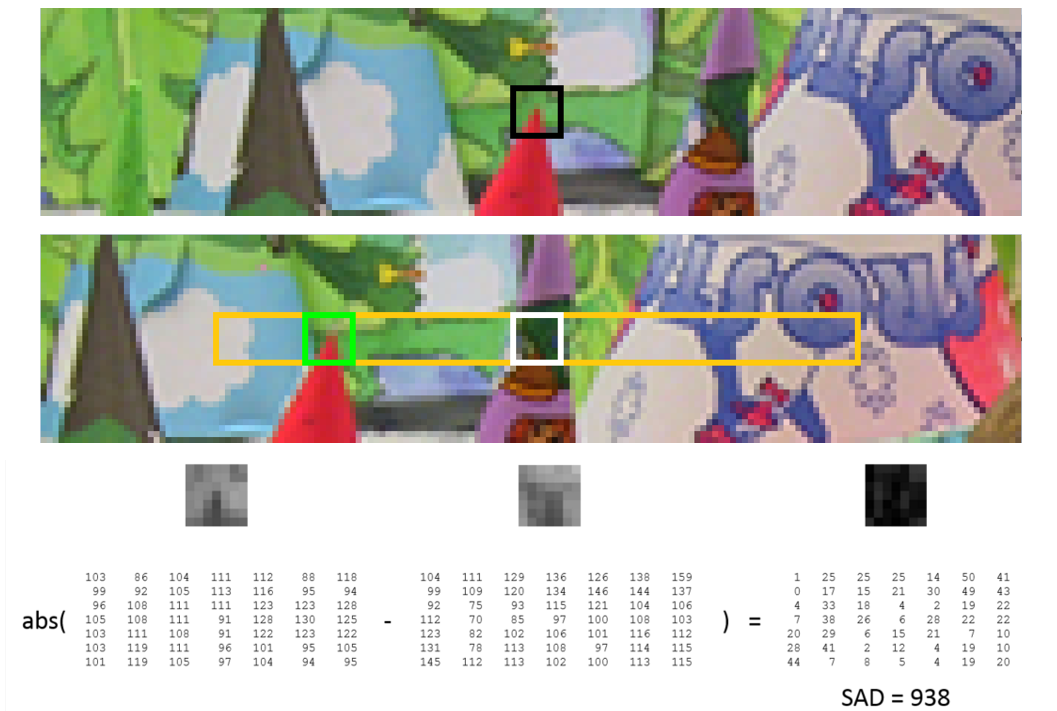
\includegraphics[width=0.75\textwidth]{SAD.PNG}}
	\caption{Sum of Absolute Differences \cite{mccormick}}
	\label{SAD}
\end{figure}
\par
Since the disparity algorithm used in this implementation calculates the sum of absolute differences for multiple search blocks, the resulting SAD values for each search block can be compared to find the location of the most similar matching block in the search image. Due to the nature of the SAD algorithm, lower SAD values indicate higher similarity between the template and search blocks. This comparison is demonstrated in Figure \ref{blockMatching} below. In the case of Figure 
ref{blockMatching}, higher match score values for each search block indicate lower SAD values.
\par
\begin{figure}[H]
	\centerline{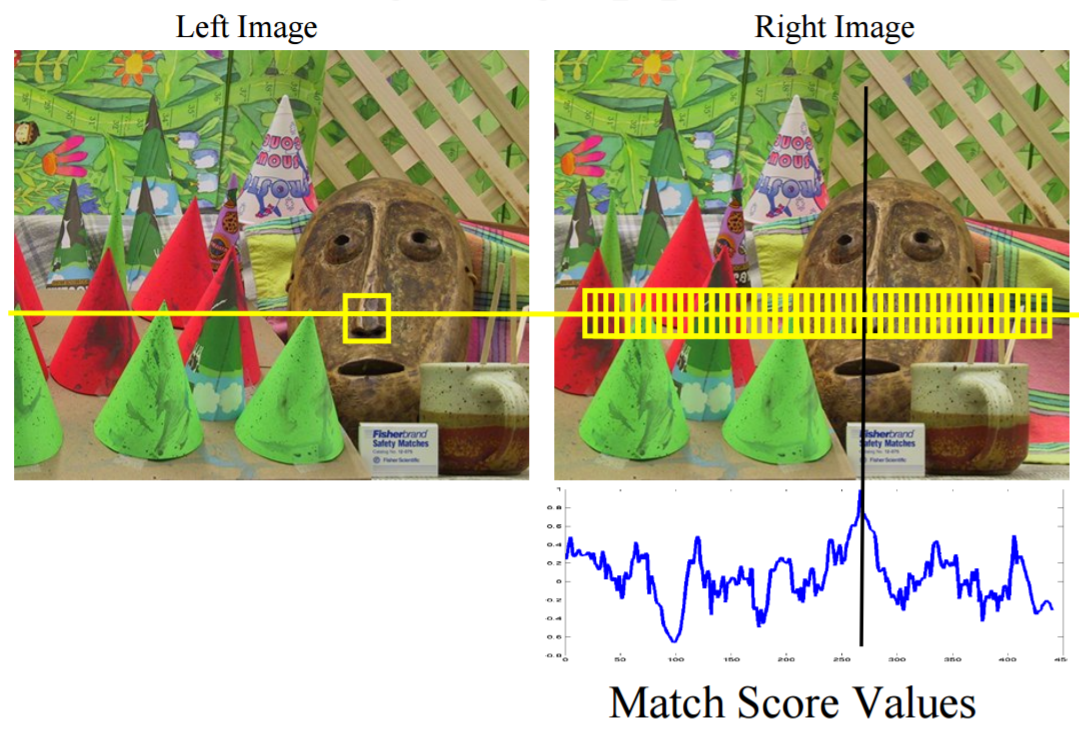
\includegraphics[width=0.75\textwidth]{blockMatching.PNG}}
	\caption{Block Matching Overview \cite{collins}}
	\label{blockMatching}
\end{figure}
\par
The SAD at multiple search points can be used to estimate the pixel offset between the template block and matching search block based on array index locations, since all SAD values for a single search are stored in a vector. This pixel offset is known as the disparity value for a given template and search block. The disparity $d$ at a given point can be transformed into a units of distance using the focal point $f$ and baseline distance $T_x$ between image sensors as shown in Equation \ref{disp2dist} below. 
\par
\begin{equation}\label{disp2dist}
depth = Z = \frac{fT_x}{d}
\end{equation}
\par
Pixel coloration values in a disparity image are based on the distance calculation shown in Equation \ref{disp2dist}, where each pixel is referenced to the disparity at a given template block's location. An example disparity image created using the \textsc{Matlab} code found in Appendix item \ref{disparityTestMatlab} is shown in Figure \ref{disparityOutput} below. 
\par
\begin{figure}[H]
	\centerline{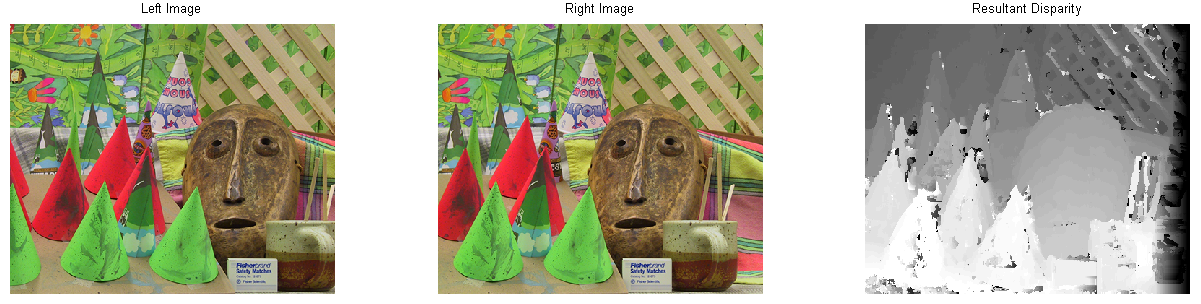
\includegraphics[width=1.1\textwidth]{disparity.png}}
	\caption{Disparity Algorithm Output}
	\label{disparityOutput}
\end{figure}

\subsubsection{Image Rectification}
The Sum of Absolute Differences algorithm operates under the assumption that objects in both camera images lie on the same horizontal line between both images, known as an epipolar line. An example of shared epipolar lines between camera imagery is shown in Figure \ref{epipolarLines} below. Although an ideal stereo camera setup would contain shared epipolar lines between camera images, raw image data from each camera will contain slight differences in object location based on the physical position of the camera modules, as well as minor differences in the lenses of each camera. Both input images can be adjusted to share the same epipolar lines through a post-processing step known as image rectification. 
\par
\begin{figure}[H]
	\centerline{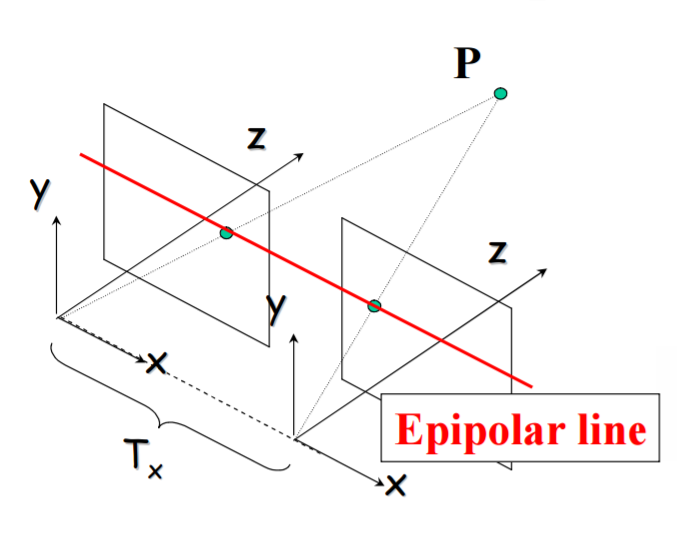
\includegraphics[width=0.75\textwidth]{epipolarLines.PNG}}
	\caption{Horizontal Epipolar Lines \cite{collins}}
	\label{epipolarLines}
\end{figure}
\par
A pictorial representation of the process of stereo image rectification is shown in Figure \ref{rectification} below \cite{mattoccia_slides}. This process is achieved using a 3x3 matrix coordinate transform based on parameters obtained from the external calibration process. 
\begin{figure}[H]
	\centerline{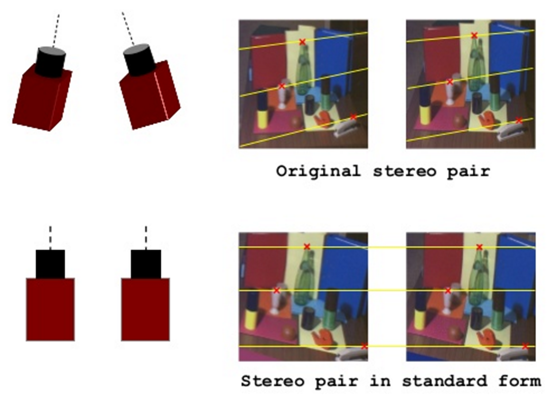
\includegraphics[width=0.75\textwidth]{rectification.png}}
	\caption{Stereo Image Rectification \cite{mattoccia_slides}}
	\label{rectification}
\end{figure}
\par
ADD AN EXAMPLE OF THE MATLAB CALIBRATION STUFF (figures showing 3d anaglyph process)

\subsubsection{Test Implementation}
The original disparity test implementation used closely follows the \textsc{Matlab} disparity algorithm shown in Appendix item \ref{disparityTestMatlab}. This algorithm is implemented using a finite state machine with five states, as shown in Figure \ref{disparityTestImp} below. In order to maintain simplicity, the test algorithm has been implemented to operate on 46x30 windowed portions of the input imagery. By default, the disparity module will remain in an idle state until an external enable signal is toggled high using a button input. This will cause the finite state machine to advance to its READ state, and image data for the left and right camera images will be read in from the stereo camera breakout board. After image data has been received, the state machine will then advance to a cyclical set of states used for iterating through each image and calculating disparity. 
\par
The disparity module will begin by isolating the template and search blocks from the right and left image data in the finite state machine's separation state. Next, the state machine will advance to its SAD state, and will calculate the sum of absolute differences between the template and search block. This value is placed in a vector that matches the length of the search range. If the vector hasn't been completely filled, indicating that there are more search blocks to compare to the template, the state machine will revert back to the separate state, isolating a new search block from the right camera image. When the SAD vector is full, the state machine will advance to its finalization state. 
\par
\begin{figure}[H]
	\centerline{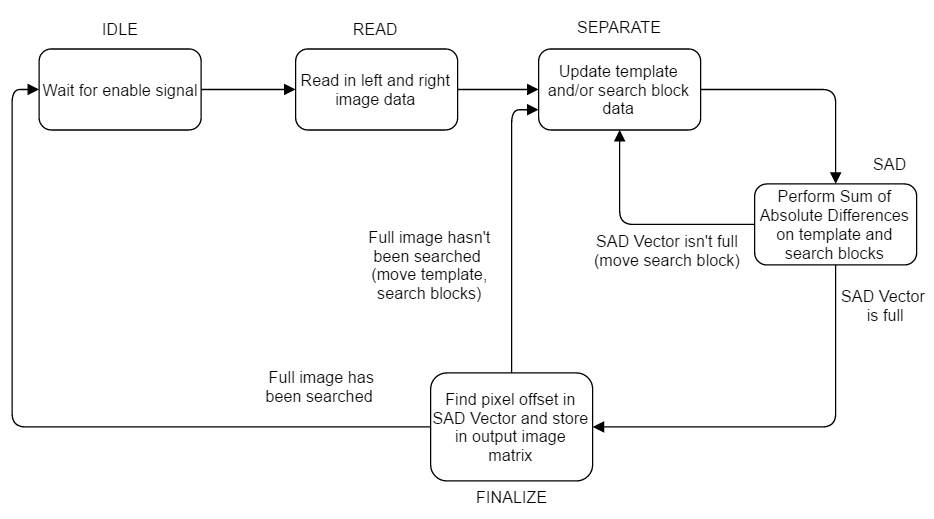
\includegraphics[width=0.75\textwidth]{looping_disparity.png}}
	\caption{Disparity Test Implementation}
	\label{disparityTestImp}
\end{figure}
\par
The finalization state is used to search through the SAD vector for the lowest value. The index of this value within the SAD vector in reference to the template block location is used to create a disparity value for the given template block location. This value is then converted to a distance using Equation \ref{disp2dist}, and is stored in the output image location. If the output image hasn't been fully populated with distance values, the state machine will then revert back to the separate state. Otherwise, the state machine will advance to its idle state, and the resulting disparity image can be read for output. 
\par
This module was initially tested using a verilog test bench, and was then tested using camera image data and a VGA display controller module, allowing for real-time verification of the algorithm's effectiveness. After testing the initial disparity algorithm, several modifications were made to increase the overall speed and efficiency of the disparity module. 

\subsubsection{Final Implementation}
\begin{figure}[H]
	\centerline{\includegraphics[width=1.2\textwidth]{Disparity_Algorithm.png}}
	\caption{Disparity Final Implementation}
	\label{disparityTestImp}
\end{figure}